% \documentclass{WHUBachelor}% 选项 forprint: 交付打印时添加, 避免彩色链接字迹打印偏淡. 即使用下一行:
\documentclass{myreport}
\usepackage[section]{placeins}
\usepackage[svgnames,table]{xcolor}
\usepackage{subfig}
\usepackage{minted}
\usepackage{tcolorbox}
\usepackage{color}
\usepackage{fancyvrb}
\newcommand{\VerbBar}{|}
\newcommand{\VERB}{\Verb[commandchars=\\\{\}]}
\DefineVerbatimEnvironment{Highlighting}{Verbatim}{commandchars=\\\{\}}
% Add ',fontsize=\small' for more characters per line
\newenvironment{Shaded}{}{}
\newcommand{\AlertTok}[1]{\textcolor[rgb]{1.00,0.00,0.00}{\textbf{#1}}}
\newcommand{\AnnotationTok}[1]{\textcolor[rgb]{0.38,0.63,0.69}{\textbf{\textit{#1}}}}
\newcommand{\AttributeTok}[1]{\textcolor[rgb]{0.49,0.56,0.16}{#1}}
\newcommand{\BaseNTok}[1]{\textcolor[rgb]{0.25,0.63,0.44}{#1}}
\newcommand{\BuiltInTok}[1]{#1}
\newcommand{\CharTok}[1]{\textcolor[rgb]{0.25,0.44,0.63}{#1}}
\newcommand{\CommentTok}[1]{\textcolor[rgb]{0.38,0.63,0.69}{\textit{#1}}}
\newcommand{\CommentVarTok}[1]{\textcolor[rgb]{0.38,0.63,0.69}{\textbf{\textit{#1}}}}
\newcommand{\ConstantTok}[1]{\textcolor[rgb]{0.53,0.00,0.00}{#1}}
\newcommand{\ControlFlowTok}[1]{\textcolor[rgb]{0.00,0.44,0.13}{\textbf{#1}}}
\newcommand{\DataTypeTok}[1]{\textcolor[rgb]{0.56,0.13,0.00}{#1}}
\newcommand{\DecValTok}[1]{\textcolor[rgb]{0.25,0.63,0.44}{#1}}
\newcommand{\DocumentationTok}[1]{\textcolor[rgb]{0.73,0.13,0.13}{\textit{#1}}}
\newcommand{\ErrorTok}[1]{\textcolor[rgb]{1.00,0.00,0.00}{\textbf{#1}}}
\newcommand{\ExtensionTok}[1]{#1}
\newcommand{\FloatTok}[1]{\textcolor[rgb]{0.25,0.63,0.44}{#1}}
\newcommand{\FunctionTok}[1]{\textcolor[rgb]{0.02,0.16,0.49}{#1}}
\newcommand{\ImportTok}[1]{#1}
\newcommand{\InformationTok}[1]{\textcolor[rgb]{0.38,0.63,0.69}{\textbf{\textit{#1}}}}
\newcommand{\KeywordTok}[1]{\textcolor[rgb]{0.00,0.44,0.13}{\textbf{#1}}}
\newcommand{\NormalTok}[1]{#1}
\newcommand{\OperatorTok}[1]{\textcolor[rgb]{0.40,0.40,0.40}{#1}}
\newcommand{\OtherTok}[1]{\textcolor[rgb]{0.00,0.44,0.13}{#1}}
\newcommand{\PreprocessorTok}[1]{\textcolor[rgb]{0.74,0.48,0.00}{#1}}
\newcommand{\RegionMarkerTok}[1]{#1}
\newcommand{\SpecialCharTok}[1]{\textcolor[rgb]{0.25,0.44,0.63}{#1}}
\newcommand{\SpecialStringTok}[1]{\textcolor[rgb]{0.73,0.40,0.53}{#1}}
\newcommand{\StringTok}[1]{\textcolor[rgb]{0.25,0.44,0.63}{#1}}
\newcommand{\VariableTok}[1]{\textcolor[rgb]{0.10,0.09,0.49}{#1}}
\newcommand{\VerbatimStringTok}[1]{\textcolor[rgb]{0.25,0.44,0.63}{#1}}
\newcommand{\WarningTok}[1]{\textcolor[rgb]{0.38,0.63,0.69}{\textbf{\textit{#1}}}}
\usepackage{longtable,booktabs}

\begin{document}
%%%%%%%%%%%%%%%%%%%%%%%%%%%%%%%%%%%%%%%%%%%%%%%%%%%%%%%%%%%%%%%%%%%%%%%%%%%%
% 封面
%%%%%%%%%%%%%%%%%%%%%%%%%%%%%%%%%%%%%%%%%%%%%%%%%%%%%%%%%%%%%%%%%%%%%%%%%%%%
% TODO: 实验标题需要修改
\title{数据库系统 \\ 酒店房间预定系统}
\Cschoolname{数据科学与计算机学院}          % 学院名
\Cmajor{计算机科学与技术}
\MyClass{计科教务二班}                 % 专业中文名
\StudentNumber{15323032,16337269,16337237} % 填写自己的学号
\author{李新锐,颜彬,王永锋}                            % 作者名字
\Csupervisor{阮文江}        %指导教师中文名、职称
\date{二〇一八年十二月二十一日}                % 日期, 要注意和英文日期一致!!
\pdfbookmark[0]{封面}{title}         % 封面页加到 pdf 书签
\maketitle
\frontmatter
%%%%%%%%%%%%%%%%%%%%%%%%%%%%%%%%%%%%%%%%%%%%%%%%%%%%%%%%%%%%%%%%%%%%%%%%%%%%
% 目录
%%%%%%%%%%%%%%%%%%%%%%%%%%%%%%%%%%%%%%%%%%%%%%%%%%%%%%%%%%%%%%%%%%%%%%%%%%%%
% 把目录加入到书签
\pagenumbering{Roman}              % 正文之前的页码用大写罗马字母编号.
\pdfbookmark[0]{目录}{toc}
\tableofcontents
%% 以下是正文
\mainmatter 
%%%%%%%%%%%%%%%%%%%%%%%%%%%%%%%%%%%%%%%%%%%%%%%%%%%%%%%%%%%%%%%%%%%%%%%%%%%%
% 正文
%%%%%%%%%%%%%%%%%%%%%%%%%%%%%%%%%%%%%%%%%%%%%%%%%%%%%%%%%%%%%%%%%%%%%%%%%%%%

% 1. 系统调查
% 2. 系统分析
% 3. 系统设计
% 4. 数据库设计
% 5. 数据库创建和数据集加载
% 6. 数据库应用软件的功能设计和开发
% 7. 数据库应用系统测试

\chapter{引言}

在本文中,我们小组对酒店客房预订管理系统进行了系统调查,分析与设计,进行了详尽的需求分析,并基于用户需求,设计了一个高效且规范的数据库模式。在此基础上,我们创建了Mysql数据库,并使用Html和Javascript编写了在线酒店客房预定管理系统。

本系统采用前后端分离的方式进行开发,前端使用了node.js及多种组件开发而成,并通过具有详尽文档的API与后端相连接,后端则完成两部分的功能,一部分是处理复杂的业务逻辑,对各种诸如注册,增添新用户,新房间,或增加新订单等接口进行处理,保证对数据库操作的一致性,另一部分是对传入API的数据进行格式检查,防止出现SQL注入或者恶意攻击API端口的情况。

在后端,除去处理复杂业务逻辑,还负责与数据库进行交互,我们编写了很多SQL查询与更新语句,在后端中根据接口传入的数据生成SQL语句,并交由数据库查询与更新。

在数据库层面,我们发现一些复杂的业务逻辑在后端编写时难以保证一致性,因此我们在数据库中编写了一些触发器与存储过程,以保证修改数据库信息时信息的一致性,对于在处理数据库数据时产生的错误,也在后端进行了适当的处理并反馈到前端中以让用户知晓。

总之,我们遵循数据库设计与网站设计与编写的方法,实现了酒店预定系统,该系统包括客房预订、会员注册、用户管理、客房管理、客户与客房的信息增删改、以及订单管理等功能,已经能够满足大多数酒店的需求。

\chapter{系统分析与设计}

随着信息化时代的到来,使用数据库来对酒店客房预订信息进行管理能够大大提高信息管理的效率。基于网络对酒店管理系统的了解,我们确定了该系统所需要满足的需求,以及我们系统应具有的功能模块。

\section{系统需求分析}

我们的系统可供酒店经理,酒店前台人员以及顾客使用。其中,不同的用户对该系统有着不同的需求,以及相应的操作权限。

对于\textbf{顾客}而言,他们需要能够在系统中:

\begin{itemize}
    \item 查询可用的房间。
    \item 预定指定的房间,提交订单。
    \item 取消自己已经订好的订单。
    \item 查看自己存在酒店中的个人信息,并且修改某些易变的项(如手机号码等)。
\end{itemize}

而对于\textbf{酒店前台人员}而言,他们不仅需要顾客本身可实现的需求,而且还应有更多信息的查询权限,更全面地说,应该如下所示:


\begin{itemize}
    \item 查询酒店所有房间的信息。
    \item 查询酒店所有订单的信息。
    \item 可能需要根据需要,取消其他用户的订单。 
    \item 增加新用户。
\end{itemize}

\textbf{酒店经理},则作为整个酒店的管理者,应当具有更多信息的修改权限,更具体的说,应该如下所示:

\begin{itemize}
    \item 增加酒店的房间类型。
    \item 酒店若新装修了房间,应当能够增加新的房间,或者修改已有的房间类型。
    \item 还需要能够对所有订单的情况做一个统计,计算酒店的营业额等信息。
\end{itemize}

\section{系统结构设计}

本系统可以分为这5个子系统,可见\autoref{fig:sub-system-design},每一个子功能都会在后端编写一个或多个对应的API供前端调用。

%\usepackage{changepage}
%\usepackage{rotating}
%\usepackage{float}
%\usepackage[section]{placeins}
%\begin{sidewaystable}[!Htp]
\begin{figure}[htp]
    %\begin{adjustwidth}{-1.5cm}{-1cm}
    \centering
    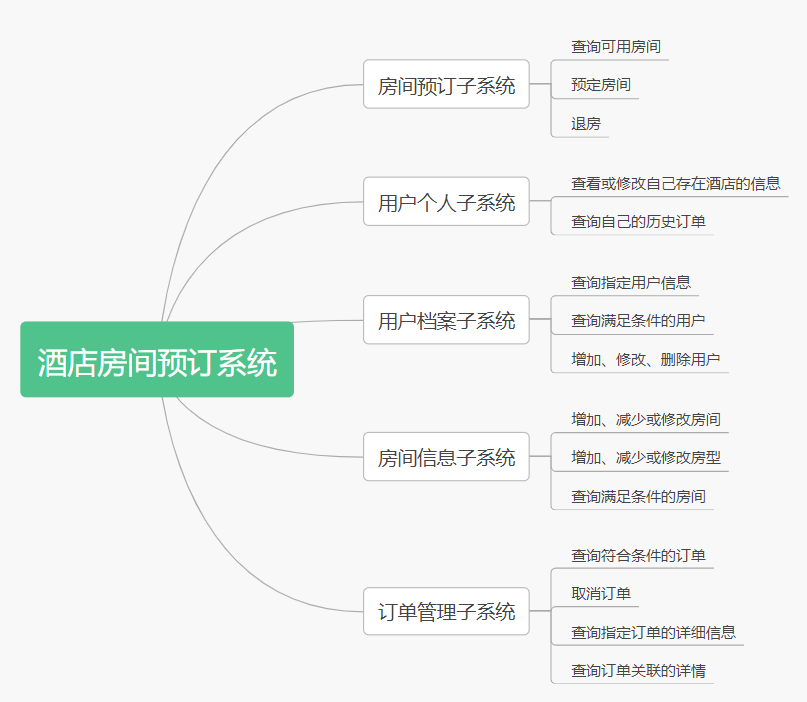
\includegraphics[width=13cm]{figure/2018-12-22-10-31-35.png}
    \caption{系统子系统设计}
    \label{fig:sub-system-design}
    %\end{adjustwidth}
\end{figure}


\chapter{数据库设计}
% TODO LXR
在本节中,我们会按照概念设计、逻辑设计到物理设计的顺序讲解本项目的具体设计方式。
\section{概念设计}

根据需求分析的结果,我们进行了数据库的概念设计,分析了数据库中应该存在的实体集、联系集,并绘制了ER图。

\subsection{实体集}



描述酒店的房间需要房间实体集(\autoref{tab:E-room})和房型实体集(\autoref{tab:E-type})。描述酒店的用户并记录用户个人和登录信息需要用户实体集(\autoref{tab:E-user})、账户实体集(\autoref{tab:E-account})、区域实体集(\autoref{tab:E-region})。
最后,酒店还需要记录所有订单(\autoref{tab:E-order}),以及订单的操作明细(\autoref{tab:E-operation})。\\

下面对这些实体集作简要的描述和区分。

\subsubsection{房间和房型实体集}

房型实体代表房内的基础设施状况,例如房内是否有wifi、是否包含早餐、容纳的人数等,可见\autoref{tab:E-type}。\\


\begin{table}[htp]
    \caption{房间实体集}
    \centering
    \rowcolors{1}{White}{Lavender}
    \begin{tabular}{cccp{11cm}<{\centering}}
    \toprule
        \emph{属性}  & \emph{备注} \\
    \midrule
        \underline{id}  & 唯一 \\
        floor & 层数\\
        room\_num  & 房间号 \\
        price & 价格  \\
    \bottomrule
    \hiderowcolors
    \end{tabular}
    \label{tab:E-room}
\end{table}


而房间实体则对应着真实的每个房间。其具有所在层数、房号、价格等属性,可见\autoref{tab:E-room}。

\begin{table}[htp]
    \caption{房型实体集}
    \centering
    \rowcolors{1}{White}{Lavender}
    \begin{tabular}{cccp{11cm}<{\centering}}
    \toprule
        \emph{属性}  & \emph{备注} \\
    \midrule
        \underline{id} & 唯一 \\
        name & 房型名称 \\
        capacity & 最大容纳人数 \\
        breakfast  & 是否包含早餐 \\
        wifi & 是否包含无线网络 \\
    \bottomrule
    \hiderowcolors
    \end{tabular}
    \label{tab:E-type}
\end{table} 

\subsubsection{用户,地区和账户实体集}

用户实体代表一个真实的个人。它有自己的身份信息,例如证件号、姓名、性别等。其中用户
实体集中的name属性代表这个人的真实姓名, 可见\autoref{tab:E-user}。\\

\begin{table}[htp]
    \caption{用户实体集}
    \centering
    \rowcolors{1}{White}{Lavender}
    \begin{tabular}{cccp{11cm}<{\centering}}
    \toprule
        \emph{属性}  & \emph{备注} \\
    \midrule
        \underline{id}  & 唯一 \\
        region & 顾客来自的地区 \\
        credential & 证件号,唯一 \\
        name & 姓名 \\
        gender & 性别 \\
        birthdate & 出生日期 \\
        phone & 电话号码 \\
    \bottomrule
    \hiderowcolors
    \end{tabular}
    \label{tab:E-user}
\end{table}

账户实体集代表本应用上的一个账号。其中的账户名(username)是登陆名,password用于
登陆。role为该账户在应用里的角色,它决定了该账户拥有的权限,可见\autoref{tab:E-account}。


\begin{table}[htp]
	\caption{账户实体集}
	\centering
	\rowcolors{1}{White}{Lavender}
	\begin{tabular}{cccp{11cm}<{\centering}}
		\toprule
		\emph{属性}  & \emph{备注} \\
		\midrule
		\underline{id}  & 唯一 \\
		username & 账户名 \\
		password & 账户密码 \\
		role & 用户角色,0为管理者,3为普通用户 \\
        balance & 余额 \\
        bonus & 积分 \\
		\bottomrule
		\hiderowcolors
	\end{tabular}
	\label{tab:E-account}
\end{table}
    

同时,为了保证每一个用户所在的地区有意义,我另外使用了一个地区实体用于确定用户所在的地区,以防止用户输入无效的地区,该实体可见\autoref{tab:E-region}。





\begin{table}[htp]
	\caption{区域实体集}
	\centering
	\rowcolors{1}{White}{Lavender}
	\begin{tabular}{cccp{11cm}<{\centering}}
		\toprule
		\emph{属性}  & \emph{备注} \\
		\midrule
		\underline{id}  & 唯一 \\
		name & 区域名称 \\
		\bottomrule
		\hiderowcolors
	\end{tabular}
	\label{tab:E-region}
\end{table}



\subsubsection{订单和操作实体集}

订单实体的信息包含了哪个用户、在何时、花费多少钱、在哪个时间段订购了哪个房间,可见\autoref{tab:E-order}。\\

\begin{table}[htp]
    \caption{订单时实体集}
    \centering
    \rowcolors{1}{White}{Lavender}
    \begin{tabular}{cccp{11cm}<{\centering}}
    \toprule
        \emph{属性} & \emph{备注} \\
    \midrule
        id & 唯一 \\
        status & 订单状态(取消、正常)\\
        check\_in & 预订的入住时间 \\
        check\_out & 预订的最后一天\\
        
    \bottomrule
    \hiderowcolors
    \end{tabular}
    \label{tab:E-order}
\end{table}


操作实体集包含了用户对订单的两种操作,分别是发起订单和取消订单,可见\autoref{tab:E-operation}。


\begin{table}[htp]
    \caption{操作明细实体集}
    \centering
    \rowcolors{1}{White}{Lavender}
    \begin{tabular}{cccp{11cm}<{\centering}}
    \toprule
        \emph{属性} & \emph{备注} \\
    \midrule
        id & 唯一 \\
        time & 操作的发生时间 \\
        detail& 操作类型(发起订单、取消订单)\\
        
    \bottomrule
    \hiderowcolors
    \end{tabular}
    \label{tab:E-operation}
\end{table}


\subsection{联系集}
房型与房间实体、房间和订单实体、用户与订单实体、区域与用户实体之间有一对多的联系。对于一个订单只有完成下单和完成下单后又取消订单两种情况,因此订单实体与订单操作实体是一对一或一对二的联系。用户与账户之间是一对一联系。
\subsection{E-R图}

\begin{figure}[H]
	\centering
	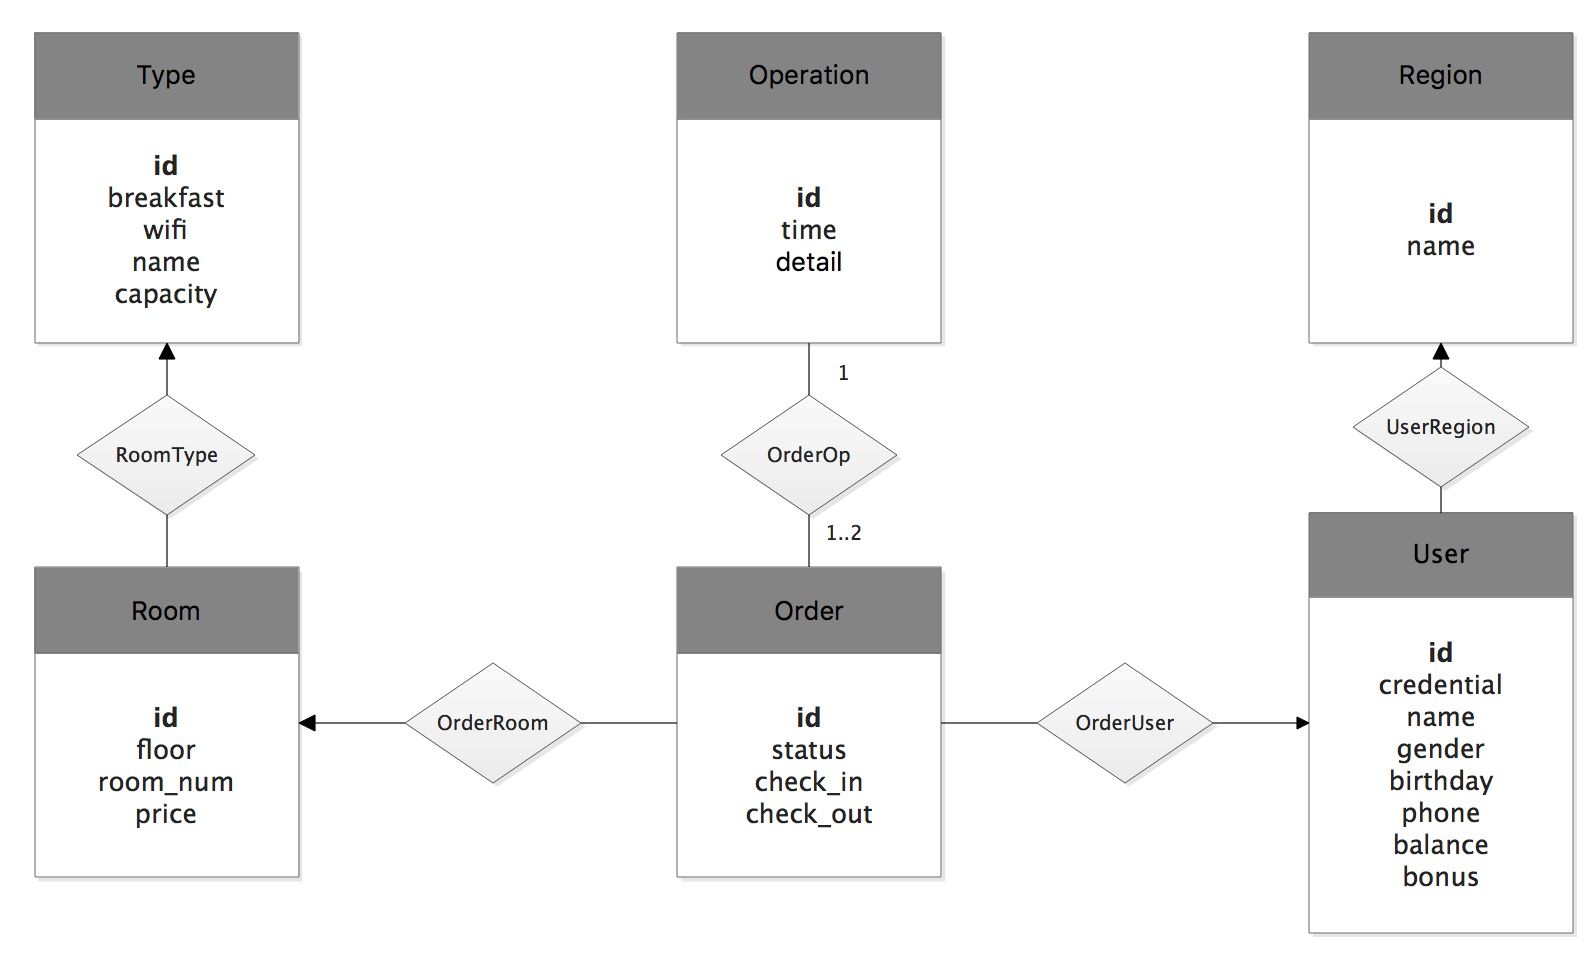
\includegraphics[width=0.9\linewidth]{../ER/project.ed.eps}
	\caption{}
	\label{fig:ER Graph}
\end{figure}

\section{逻辑设计}

在完成数据库的概念设计后,接下来要做的是将所有实体集合联系集分别转换为关系模式$R$。

有关实体集的转换规则如下:

\begin{itemize}
	\item 具有$n$个简单描述性属性的强实体集转换为具有$n$个属性的关系模式
	\item 为复合属性的每个子属性在$R$中创建一个单独的属性
	\item 为多值属性$M$创建一个单独的关系模式,该模式中包含了$M$所在的实体集或联系集的主码
	\item 将派生属性实现为方法
	\item 将弱实体集表示为包含所有弱实体集属性以及所依赖的强实体集的主码的关系模式。$R$的主码包括弱实体集的部分码和所以来的强实体集的主码。
\end{itemize}

有关联系集的转换规则如下:

\begin{itemize}
	\item 联系集转换为由联系集的描述性属性以及相关实体集的主码组成的关系模式
	\item 对于多对多的联系集,$R$的主码包含所有相关实体集的主码
	\item 对于一对一的联系集,任意一个相关实体集的主码都可以作为$R$的主码
	\item 对于一对多的联系集,用关联的映射基数为"多"的那个实体集作为$R$的主码
\end{itemize}

转换完成后,还要消除关系模式的冗余,并合并部分关系模式。具体而言包括以下两种情况:

\begin{itemize}
	\item 连接弱实体集与其依赖的强实体集的联系集的模式是多对一且没有描述性属性的,另外弱实体集的主码包含强实体集的主码,因此这样的联系集对应的关系模式是冗余的。
	\item 考虑多对一的联系集$AB$和相关的实体集$A$, $B$, ,若$A$在联系中的参与是全部的,那么可以将$A$与$AB$模式属性合并得到$A^*$,主码是$A$的主码,外码加入$A^*$中。
\end{itemize}

依照上述规则,由于Type、Room、Operation、Order、User、Region、Account均为简单强实体集于是可以首先生成包含对应属性的关系模式。再考虑联系集,由于OrderUser、RoomType、OrderRoom、OrderOp、UserRegion均为一对多的联系集,因此均可以按照上述规则消除。

最后得到以下关系模式:

RoomType(\textbf{id}, name, capacity, breakfast, wifi)

Room(\textbf{id}, floor, room\_num, price, \textit{type\_id})

Operation(\textbf{id}, time, detail. \textit{order\_id})

Order(\textbf{id}, status, check\_in, check\_out, \textit{room\_id}, \textit{user\_id})

Region(\textbf{id}, name)

User(\textbf{id}, credential, name, gender, birthdate, phone, bonus, balance, \textit{region\_id})

Account(\textit{\textbf{id}}, username, password, role)


\section{物理设计}
% TODO: YB 颜彬

在这一部分中,我们主要对数据库中索引的设计做了一个比较详细的解释,说明了我们对数据库性能问题的考虑与我们的解决方案。

\subsection{索引简介}
在MariaDB中,有4种类型的索引(Mariadb不严格地区分key和index的概念,
并时常根据语境对他们混用)。\\

\autoref{tab:index}列出了这4种索引。 其中unique表示索引建立的数据项
是否必须唯一,not null表示数据项是否必须不为null。\\

mariaDB会自动为primary key 和 foreign key建立索引(表第一行)。
其中如果对unique的数据项建立索引,可以建立一个unique索引(表第二行)。
如果该数据项不是唯一的,则需要建立plain indexes或full-text indexes。
后两者最大的不同在于,如果使用like `\%word\%'这种形式的查询,必须建立
full-text索引,否则无效。

\begin{table}[htp]
    \caption{mariaDB索引介绍}
    \centering
    \rowcolors{1}{White}{Lavender}
    \begin{tabular}{cccp{11cm}<{\centering}}
    \toprule
        \emph{名称} & \emph{unique} & \emph{not null} \\
    \midrule
        primary(foreigh) key & Y & Y \\
        unique indexes & Y & N \\
        plain indexes & N & N \\
        full-text indexes & N & N \\
    \bottomrule
    \hiderowcolors
    \end{tabular}
    \label{tab:index}
\end{table}
\subsubsection{索引建立}
搜索订单几乎是最常见的一种操作。从用户的行为来判断,大部分对订单的搜索都是基于订单日期的。
故在Order表上对check\_in和check\_out添加索引十分有必要。\\

%\usepackage{minted}
%\inputminted{c}{hello.c}
%\fontsize=\footnotesize
%use the complie option: --shell-escape
\begin{minted}[mathescape, linenos, numbersep=5pt, gobble=4, frame=lines, framesep=2mm,breaklines, breakafter=d,fontsize=\footnotesize,escapeinside=||]{sql}
    CREATE INDEX Order__index_check_in ON `Order` (check_in DESC);    
\end{minted}


在上面的索引建立中,显式地指明了索引使用降序排列。
这是因为根据时间局部性,越``晚(刚刚发生)''的记录越可能被搜索,越``早(年代久远)''
的记录越不可能被搜索。降序排列索引可以尽可能早地让索引被搜索到。\\

\subsection{效果评价}

%\usepackage{minted}
%\inputminted{c}{hello.c}
%\fontsize=\footnotesize
%use the complie option: --shell-escape
\begin{minted}[mathescape, linenos, numbersep=5pt, gobble=4, frame=lines, framesep=2mm,breaklines, breakafter=d,fontsize=\footnotesize,escapeinside=||]{sql}
explain 
select * from `Order`
where check_in >= '2019-01-22';
\end{minted}


比较有索引和无索引时的相关输出。
没有建立索引时,仅能根据主键索引进行查询。查询了300多行。
但建立了对check\_in的索引后,以上的语句仅需要搜索75行,大大加快了搜索时间。\\

进一步测试以下的语句\\

%\usepackage{minted}
%\inputminted{c}{hello.c}
%\fontsize=\footnotesize
%use the complie option: --shell-escape
\begin{minted}[mathescape, linenos, numbersep=5pt, gobble=4, frame=lines, framesep=2mm,breaklines, breakafter=d,fontsize=\footnotesize,escapeinside=||]{sql}
    explain select * from `Order`
    where check_in >= '2019-01-22'
    AND check_out <= '2020-01-01';
\end{minted}


发现mariaDB的做法是,先根据索引check\_in作range scan,估计会检索到75个左右的行。
然后对这些行作where筛选,得到最终的结果。\\

在上面的语句执行中,没有用到check\_out索引,但这个索引依旧有它的必要指之处。
mariaDB会选择check\_in或check\_out中的一个索引作range scan,很
可能在下一次更合适的情况下会使用check\_out。维护check\_in和check\_out两个索引,
可以让mariaDB有更多提升性能的可能性。\\

更进一步的分析,如果用户想要筛选订单,必行会出现user\_id = <int>的情况。
此时user\_id一定是更适合的索引。但不能忽略的是,酒店的前台也需要筛选订单。
后者往往是根据日期作筛选的,而且这个操作的发生极其频繁。故这个索引十分有必要。\\

\subsection{其他索引的需求分析}
大部分对User表的查询都是使用id进行查询的。user name是用户的真名,
对用户真名的查询操作其实很少。故现有的主键索引已经足够。\\

对Account的查询中,由于username被标记为unique(IDE自动为我们建立了索引),
故对Account的大部分查询效率都很高。\\

一个比较微妙的操作是查询空闲房间。因为查询空闲房间涉及到查询房间(Room)、
查询房间类型(RoomType)和查询订单(Order)三个表的数据。
实际上这个操作的效率也是很高的。对此详细的介绍见后文。\\


我们的应用经常需要返回``空闲的房间数''。可是怎么定义空闲呢?
如果对于一段查询时间[check\_in, check\_out],不存在与之重叠的订单(order),
那么我们就说这个房间是空闲的。
但实际的查询并不是通过使用check\_in和check\_out的索引进行的。\\

%\usepackage{minted}
%\inputminted{c}{hello.c}
%\fontsize=\footnotesize
%use the complie option: --shell-escape
\begin{minted}[mathescape, linenos, numbersep=5pt, gobble=4, frame=lines, framesep=2mm,breaklines, breakafter=d,fontsize=\footnotesize,escapeinside=||]{sql}
    explain 
    select R.id, R.floor, R.room_num, R.price, T.breakfast, T.wifi ,T.name, T.capacity
    from Room as R, RoomType as T
    where R.type_id = T.id
      and T.capacity >= 2
      and T.wifi like 1
      and T.breakfast like 1
      and not exists
        ( select room_id, O.id
          from `Order` as O
          where status = 1
            and ((O.check_in <= '2018-11-20' and O.check_out >= '2018-12-30')
              or (O.check_in <= '2018-10-30' and O.check_out >= '2018-11-10'))
            and O.room_id = R.id );
\end{minted}

使用explain查看查询计划后,我们发现,mariaDB
\begin{itemize}
    \item 首先使用where筛选掉不符合要求的RoomType。
    由于RoomType是很小的一个表,这一步的效率非常高。
    \item 利用Room对RoomType的外键索引筛选合适的Room。
    由于利用了索引,这一步速度也非常高。
    \item 利用Order对Room的外键索引筛选合适的Order。
    由于利用了索引,这一步的速度也非常高。
\end{itemize}
  
这说明我们没有额外建立索引的必要了,现有的主键和外键索引已经能让数据库的执行速度足够高了。\\


只有订单的check\_in和check\_out需要额外的索引。
其他操作都可以通过主键外键索引、unique索引得到加速。


\chapter{数据库创建和数据加载}
%TODO: LXR
\section{视图}
在酒店管理系统中,为了对账需要,所有历史订单都不能删除。但用户通常只关心还未退房的订单,系统在查询空房时,也
只是对照那些还没退房的订单使用排除法进行查找。因此,保存一个仅包含还未退房的订单的视图能够方便数据库后台的管理和应用的实现,视图实现的代码如下。

%\usepackage{minted}
%\inputminted{c}{hello.c}
%\fontsize=\footnotesize
%use the complie option: --shell-escape
\begin{minted}[mathescape, linenos, numbersep=5pt, gobble=4, frame=lines, framesep=2mm,breaklines, breakafter=d,fontsize=\footnotesize,escapeinside=||]{sql}
    create view VIEW_available_orders as
    select *
      from `Order` o
      where o.status = 1 and o.check_out > CURDATE();
\end{minted}


\section{存储过程}

\label{procedure}

\subsection{查询可用房间}

在酒店管理系统中,我们不可能存储未来每一天每间房间是否可用的状态。要查询某个指定时间段空闲的房间有哪些,必须根据当前有效的订单信息,查询并排除该时间段内已经被预定的房间。由于查询可用房间是酒店数据库最常用的功能,因此我们设计了存储过程:


%\usepackage{minted}
%\inputminted{c}{hello.c}
%\fontsize=\footnotesize
%use the complie option: --shell-escape
\begin{minted}[mathescape, linenos, numbersep=5pt, gobble=4, frame=lines, framesep=2mm,breaklines, breakafter=d,fontsize=\footnotesize,escapeinside=||]{sql}
    create procedure PROC_find_avail_room
    (in Arg_check_in Date, in Arg_check_out Date, 
     in Arg_capacity int, in Arg_wifi char(1), in Arg_breakfast char(1))
    begin
    select R.id,R.floor, R.room_num,R.price, 
    T.breakfast, T.wifi ,T.name, T.capacity
    from Room as R, RoomType as T
    where R.type_id = T.id and T.capacity >= Arg_capacity 
    and T.wifi like Arg_wifi and T.breakfast like Arg_breakfast and
    (not exists (select * from VIEW_available_orders o
        where  R.id = o.room_id and Arg_check_in <= o.check_out and 
                 Arg_check_out >= o.check_in
    ));
    end;
\end{minted}

该存储过程的参数说明可见\autoref{tab:query_avail_room-arg}。

%\usepackage[svgnames,table]{xcolor}
%\usepackage{changepage}
%\usepackage{rotating}
%\begin{sidewaystable}[htp]
\begin{table}[htp]
    \caption{查询可用房间-参数说明}
    \centering
    \rowcolors{1}{White}{Lavender}
    %\begin{adjustwidth}{-1.5cm}{-1cm}
    \begin{tabular}{ccc}
%\multicolumn{2}{c}{contents}
%\usepackage{booktabs}
%\cmidrule{2-3}
    \toprule
        参数 & 类型 & 值 \\
    \midrule
     Arg\_check\_in  & Date    & 预约的第一天         \\
     Arg\_check\_out & Date    & 预约的最后一天       \\
     Arg\_capacity  & int     & 预约的房型的最低容量 \\
     Arg\_wifi      & char(1) & 是否要求要WiFi       \\
     Arg\_breakfast & char(1) & 是否要求送早餐       \\
    \bottomrule
    \hiderowcolors
    \end{tabular}
    %\end{adjustwidth}
    \label{tab:query_avail_room-arg}
\end{table}

可以通过以下方式调用该存储过程,表示查询入住时间为2019年1月22日,退房时间也为2019年1月22日测情况下,有wifi且可住两人的空闲房间。

%\usepackage{minted}
%\inputminted{c}{hello.c}
%\fontsize=\footnotesize
%use the complie option: --shell-escape
\begin{minted}[mathescape, linenos, numbersep=5pt, gobble=4, frame=lines, framesep=2mm,breaklines, breakafter=d,fontsize=\footnotesize,escapeinside=||]{sql}
    call PROC_find_avail_room('2019-01-22', '2019-01-22', 2, '1', '%');
\end{minted}

\subsection{预定房间}

预定房间在系统中设计多个操作,首先要在数据库中查询该房间是否可被预定,然后如果没有被预定,则需要在Order表中生成一个新订单,然后在Operation表中生成一条该订单的生成记录,同时还需要扣除指定用户余额,这一连串的操作应当以事务的形式来实现,因此我们将整个复杂的过程,使用存储过程在数据库中实现,代码可见如下:

%\usepackage{minted}
%\inputminted{c}{hello.c}
%\fontsize=\footnotesize
%use the complie option: --shell-escape
\begin{minted}[mathescape, linenos, numbersep=5pt, gobble=0, frame=lines, framesep=2mm,breaklines, breakafter=d,fontsize=\footnotesize,escapeinside=||]{sql}
create or replace procedure PROC_order_room
(in Arg_room_id int, in Arg_user_id int, in Arg_check_in Date, in Arg_check_out Date)
begin
    declare L_price integer ;
    declare L_days integer ;
    declare L_already_occupied integer ;
    select (DATEDIFF(Arg_check_out, Arg_check_in)+1) into L_days;
    start transaction ;
    select count(o.id) from VIEW_available_orders o
    where Arg_room_id = o.room_id and Arg_check_in <= o.check_out and Arg_check_out >= o.check_in
    into L_already_occupied;
    IF (L_already_occupied) THEN
    SIGNAL SQLSTATE '45000' SET
    MYSQL_ERRNO = 30004,
    MESSAGE_TEXT = 'Sorry, the room is already occupied';
    elseif (L_days < 0) THEN
    SIGNAL SQLSTATE '45000' SET
    MYSQL_ERRNO = 30001,
    MESSAGE_TEXT = 'Wrong order(Arg_check_in > Arg_check_out)';
    else
    select r.price from Room r
    where r.id = Arg_room_id
    into L_price;
    insert into `Order` (room_id, user_id, check_in, check_out, status,fee) value
    (Arg_room_id, Arg_user_id, Arg_check_in, Arg_check_out, 1, L_price * L_days);
    insert into Operation(time, detail, order_id) value( now(), 1, LAST_INSERT_ID());
    end if;
    commit;
end;  
\end{minted}

该存储过程的参数说明可见\autoref{tab:order_room-arg}。

%\usepackage[svgnames,table]{xcolor}
%\usepackage{changepage}
%\usepackage{rotating}
%\begin{sidewaystable}[htp]
\begin{table}[htp]
    \caption{预定房间-存储过程}
    \centering
    \rowcolors{1}{White}{Lavender}
    %\begin{adjustwidth}{-1.5cm}{-1cm}
    \begin{tabular}{ccc}
%\multicolumn{2}{c}{contents}
%\usepackage{booktabs}
%\cmidrule{2-3}
    \toprule
        参数 & 类型 & 值 \\
    \midrule
     Arg\_room\_id   & int  & 想预订的房间id \\
     Arg\_user\_id   & int  & 进行预订的用户 \\
     Arg\_check\_in  & Date & 预约的入住时间 \\
     Arg\_check\_out & Date & 预约的最后一天 \\
    \bottomrule
    \hiderowcolors
    \end{tabular}
    %\end{adjustwidth}
    \label{tab:order_room-arg}
\end{table}

\subsection{退房}

退房操作同样涉及到较多的操作,首先需要判断该房间是否已经预定,只有已经预定了的房间才能够被取消;在确定能够退房后,需要以事务的方式完成以下的一连串操作:在Order表中将指定订单的状态设置为取消,然后计算退房费用并返还到用户账户中,同时还需要在Operation表中生成一条新纪录,记录该订单的取消操作。以事务的方式完成上述一系列操作能够保证数据库中数据的一致性。

该存储过程的代码可见如下,只需要为该存储过程提供订单编号即可进行操作。

%\usepackage{minted}
%\inputminted{c}{hello.c}
%\fontsize=\footnotesize
%use the complie option: --shell-escape
\begin{minted}[mathescape, linenos, numbersep=5pt, gobble=0, frame=lines, framesep=2mm,breaklines, breakafter=d,fontsize=\footnotesize,escapeinside=||]{sql}
create procedure PROC_cancel_order(IN Arg_order_id int)
begin
    declare O_status int;
    declare O_check_in Date;
    declare O_check_out Date;
    declare O_refund_days int;
    select -1 into O_status;
    select O.status from VIEW_available_orders O
    where O.id = Arg_order_id
    into O_status;
    select O.check_in
    from VIEW_available_orders O
    where O.id = Arg_order_id
    into O_check_in;
    select O.check_out
    from VIEW_available_orders O
    where O.id = Arg_order_id
    into O_check_out;
    IF (CURDATE() >= O_check_out or O_status = 0 or O_status = -1) THEN
    SIGNAL SQLSTATE '45000' SET
    MYSQL_ERRNO = 30005,
    MESSAGE_TEXT = 'Sorry, cancelling this order is not available';
    elseif (CURDATE() < O_check_in) Then
    start transaction;
    update User, `Order`
    set User.balance = User.balance + `Order`.fee
    where `Order`.id = Arg_order_id and `Order`.user_id = User.id;
    update `Order`
    set `Order`.status = 0
    where `Order`.id = Arg_order_id;
    insert into Operation(time, detail, order_id)
    value (now(), 2, Arg_order_id );
    commit;
    else
    start transaction;
    select DATEDIFF(O_check_out, CURDATE())
    into O_refund_days;
    update User, `Order`
    set User.balance =
        User.balance + O_refund_days *
        `Order`.fee /(O_check_out - O_check_in + 1)
        where User.id = `Order`.user_id and `Order`.id = Arg_order_id;
    update `Order`
    set `Order`.status = 0
    where `Order`.id = Arg_order_id;
    insert into Operation(time, detail, order_id) value (now(), 2, Arg_order_id);
    commit ;
    end if;
end;
\end{minted}

\section{建立触发器}
用户每次订房时要从余额中扣取房费并给予积分奖励,这一操作必须在订单生成前完成,并对用户余额进行检查,避免用户余额不足,该触发器的实现可见以下代码:

%\usepackage{minted}
%\inputminted{c}{hello.c}
%\fontsize=\footnotesize
%use the complie option: --shell-escape
\begin{minted}[mathescape, linenos, numbersep=5pt, gobble=0, frame=lines, framesep=2mm,breaklines, breakafter=d,fontsize=\footnotesize,escapeinside=||]{sql}
create or replace trigger TRI_order_fee
    before insert on `Order`
   for each row
   begin
   declare fee integer;
   declare days integer;
   declare old_balance integer ;
   select balance into old_balance
   from User u
   where  u.id = New.user_id;
   IF (old_balance = null or old_balance - New.fee < 0) THEN
    SIGNAL SQLSTATE '45000' SET
    MYSQL_ERRNO = 30001,
    MESSAGE_TEXT = 'You dont have enough balance';
   else
    update User u
    set balance = old_balance - New.fee
    where u.id = NEW.user_id;
   END IF;
   end;
\end{minted}



\section{事务机制}
出于安全性考虑,我们将用户的账户与用户的个人信息分在两个表中分开存储。而酒店一般要求用户实名制登记,因此在注册时不仅要在账户表中添加账户,而且一定要在用户信息表相应地记录真实姓名和证件号码。为了确保用户注册操作的原子性,我们采用了事务机制,将两次插入操作在一次事务中提交。

通过,对订单的操作同样也采用了事务机制,“修改用户余额”,“生成订单”,“生成订单操作明细”三个操作的执行必须一一整个事务的方式来执行,否则可能会出现不一致的情况。

这一部分的代码实现,可见\autoref{procedure}存储过程一节。

\section{自主存取控制}
为了防止用户账户失窃、账单等数据因操作不当丢失,我们设计了自主存取控制机制,将数据库后台人员分为管理员和审计员,对用户权限进行如下分配: 
\begin{itemize}
    \item 只有管理员有查看和修改Account表的权限
    \item 审计员对其他表只有查看权限
    \item 管理员对Order表有除了delete、alter、delete history之外的其他权限
    \item 管理员对其他表有所有权限
\end{itemize}

\section{测试数据生成}

在这一步,我使用了python编写生成数据的脚本,并在其中对表中已存在的约束做了适当的控制,保证初始化的数据在数据库中是一致的。具体而言,我关注到了以下细节:

\begin{itemize}
    \item Room表中的type\_id,受到RoomType表中id一列的外键约束。
    \item Account表中的id,受到User表中id一列的外键约束。
    \item Order表中的user\_id,room\_id,均受到User表id与Room表id的外键约束。
    \item Order表中预约成功的订单,在Operation表中应有一条对应的生成订单记录。
    \item Order表中预约失败的订单,在Operation表中应有两条对应的订单操作记录,一条为生成,另一条为取消。
\end{itemize}

测试数据示例可见\autoref{fig:test-data}

%\usepackage{changepage}
%\usepackage{rotating}
%\usepackage{float}
%\usepackage[section]{placeins}
%\begin{sidewaystable}[!Htp]
\begin{figure}[htp]
    %\begin{adjustwidth}{-1.5cm}{-1cm}
    \centering
    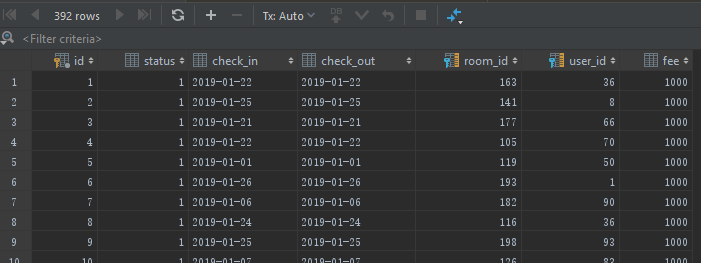
\includegraphics[width=12cm]{figure/2018-12-22-15-36-08.png}
    \caption{测试数据示例}
    \label{fig:test-data}
    %\end{adjustwidth}
\end{figure}


关于生成数据相关的python代码,由于与该系统设计关系不大,因此不放在报告中呈现。

\chapter{数据库应用软件设计开发与测试}

\section{系统整体架构}

我们系统设计采用了前后端分离的模式,具体可见\autoref{fig:system-arch}。


% 画一幅图,说明 前端, 后端 ,数据库之间的交互关系
%\usepackage{changepage}
%\usepackage{rotating}
%\usepackage{float}
%\usepackage[section]{placeins}
%\begin{sidewaystable}[!Htp]
\begin{figure}[htp]
    %\begin{adjustwidth}{-1.5cm}{-1cm}
    \centering
    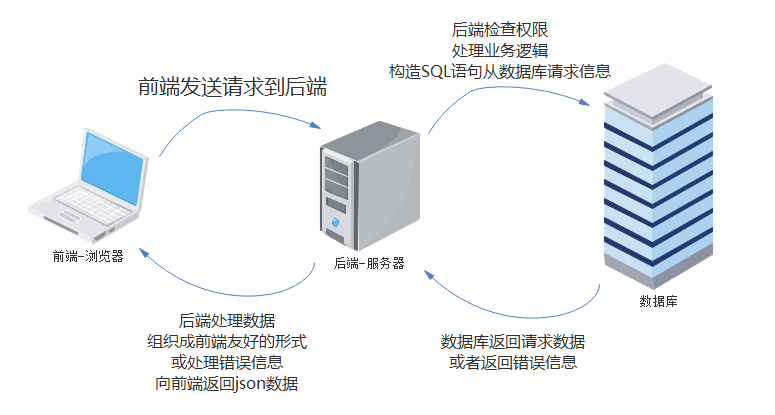
\includegraphics[width=13cm]{figure/2018-12-22-12-09-07.png}
    \caption{系统整体架构}
    \label{fig:system-arch}
    %\end{adjustwidth}
\end{figure}

\section{后端API设计}


关于后端的API设计,我们编写了一份完整且规范的API文档,其中含有每一个API的参数说明,返回值,以及错误信息的设置,文档将会在项目中另外附上一份文件进行说明,截图可见\autoref{fig:api-document-example}:

%\usepackage{changepage}
%\usepackage{rotating}
%\usepackage{float}
%\usepackage[section]{placeins}
%\begin{sidewaystable}[!Htp]
\begin{figure}[htp]
    %\begin{adjustwidth}{-1.5cm}{-1cm}
    \centering
    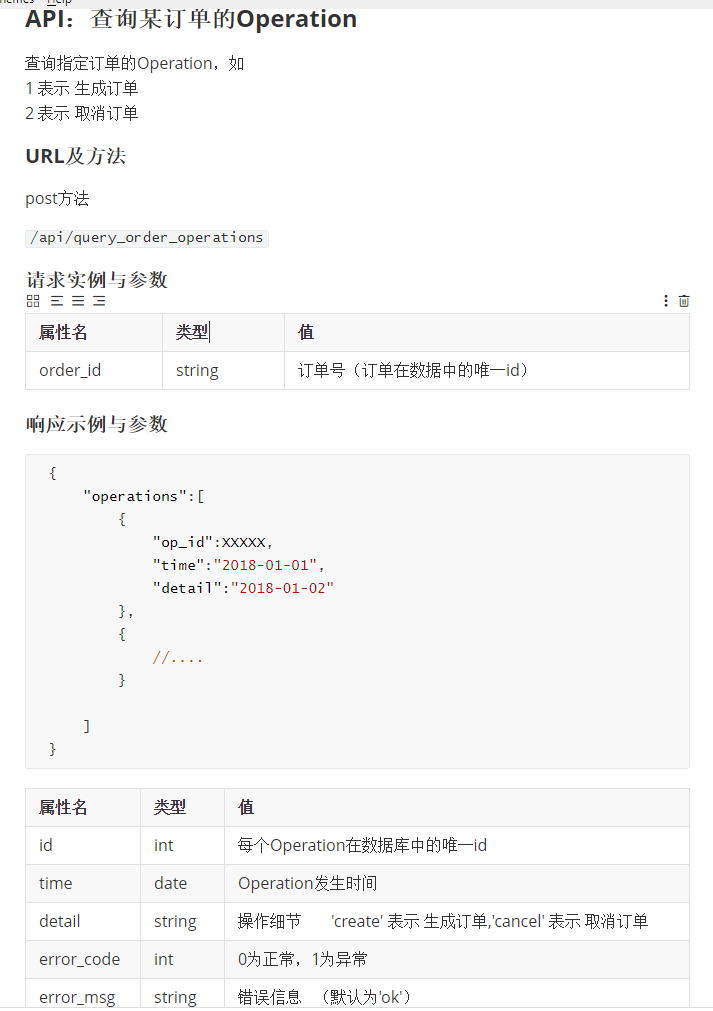
\includegraphics[width=13cm]{figure/2018-12-22-12-14-27.png}
    \caption{后端API文档示例}
    \label{fig:api-document-example}
    %\end{adjustwidth}
\end{figure}


\section{系统界面说明}

% 截图,说一下系统各部件的作用啥的
关于系统的界面,需要注意到,酒店经理所看到的系统界面与用户所看到的的系统界面应当是不同的,用户界面可见\autoref{fig:user-mode},酒店经理使用界面可见\autoref{fig:admin-mode}。


%\usepackage{changepage}
%\usepackage{rotating}
%\usepackage{float}
%\usepackage[section]{placeins}
%\begin{sidewaystable}[!Htp]
\begin{figure}[htp]
    %\begin{adjustwidth}{-1.5cm}{-1cm}
    \centering
    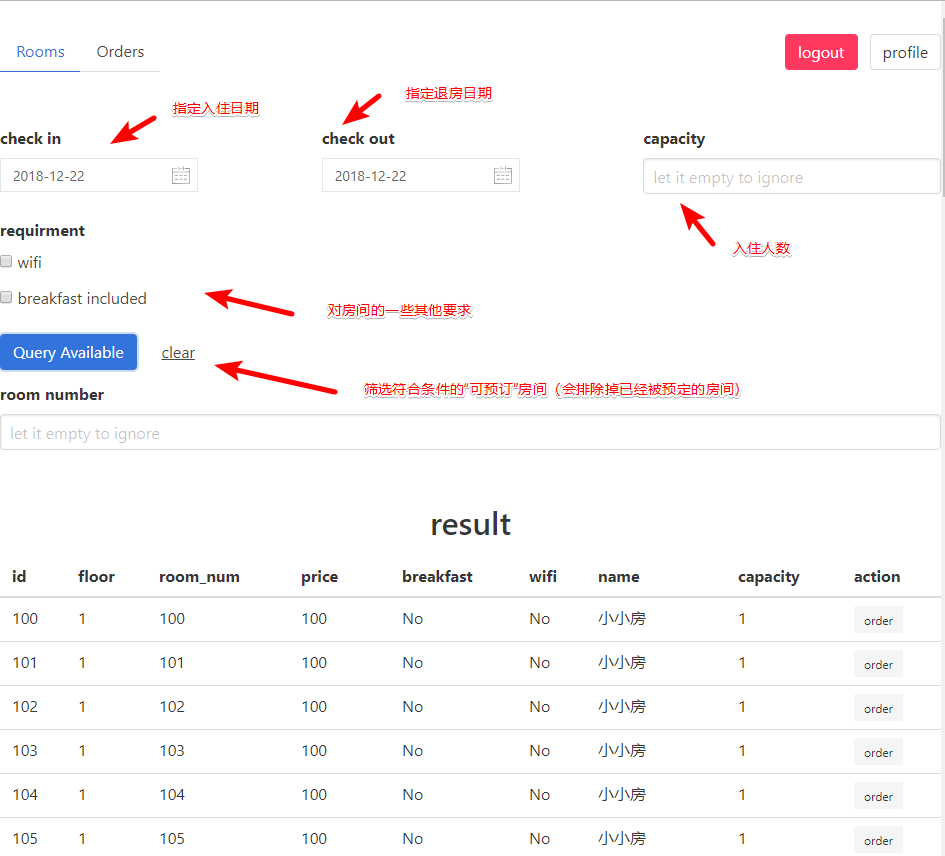
\includegraphics[width=15cm]{figure/2018-12-22-14-57-11.png}
    \caption{用户界面}
    \label{fig:user-mode}
    %\end{adjustwidth}
\end{figure}

%\usepackage{changepage}
%\usepackage{rotating}
%\usepackage{float}
%\usepackage[section]{placeins}
%\begin{sidewaystable}[!Htp]
\begin{figure}[htp]
    %\begin{adjustwidth}{-1.5cm}{-1cm}
    \centering
    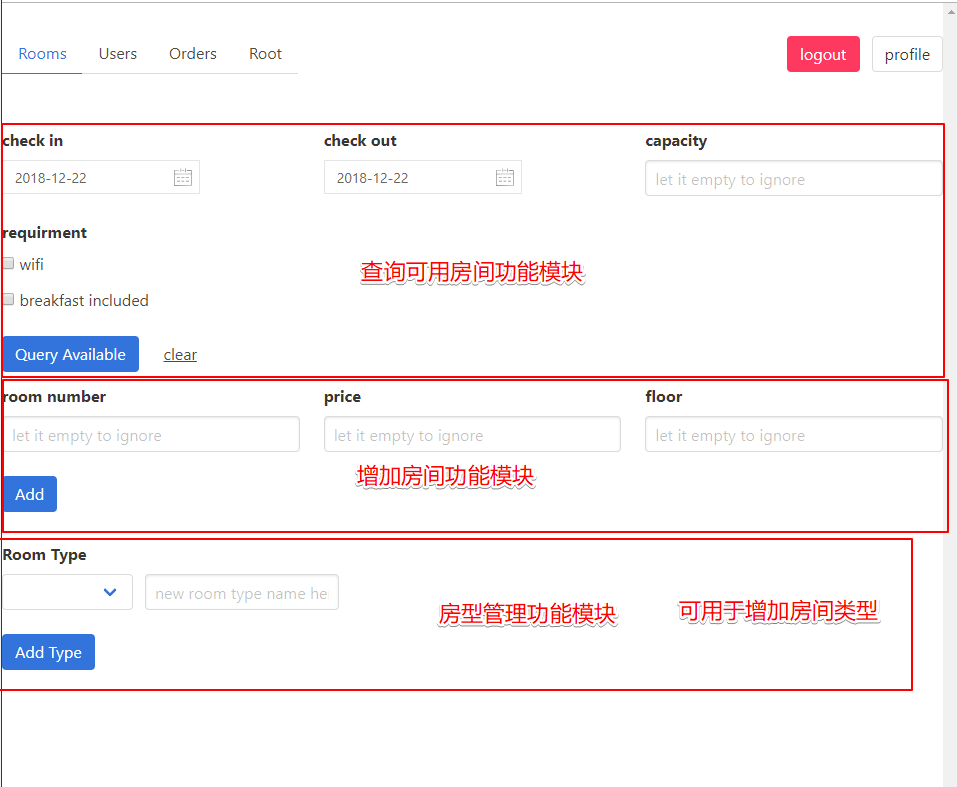
\includegraphics[width=15cm]{figure/2018-12-22-15-00-55.png}
    \caption{酒店经理使用界面}
    \label{fig:admin-mode}
    %\end{adjustwidth}
\end{figure}



\chapter{系统测试}

在这一部分,我演示了一个在本系统中比较典型的操作,用户预订房间与查询取消订单,更详细的说明可见报告附件中的屏幕录像文件。

\section{用户预订房间}

一个用户名为“123”的用户要预订“2019-01-01”-“2019-01-09”的至少能住5人的房间,因此他打开了该酒店房间预订系统,并使用用户名“123”,密码“123”登录进入系统,并选择对应的房间。

%\usepackage{changepage}
%\usepackage{rotating}
%\usepackage{float}
%\usepackage[section]{placeins}
%\begin{sidewaystable}[!Htp]
\begin{figure}[htp]
    %\begin{adjustwidth}{-1.5cm}{-1cm}
    \centering
    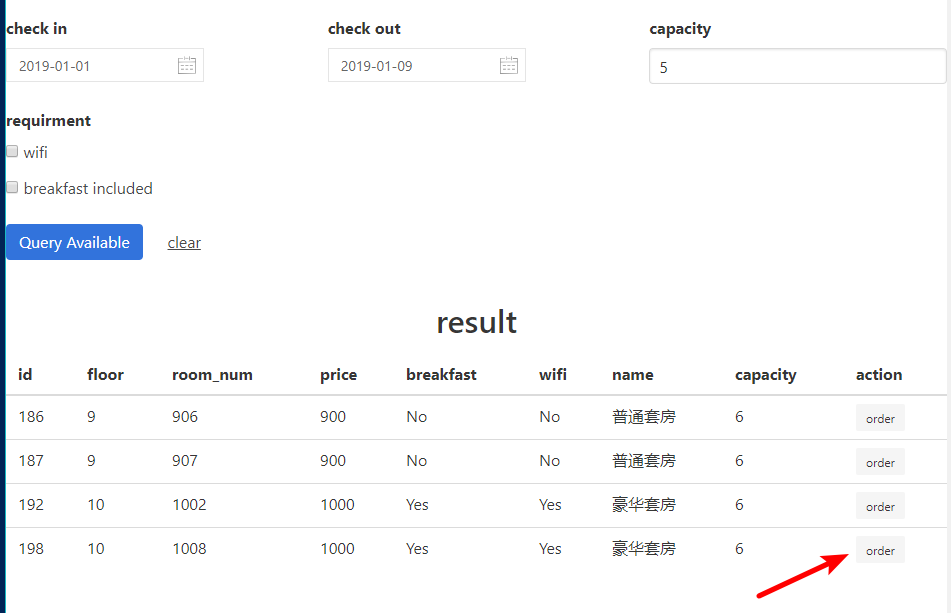
\includegraphics[width=15cm]{figure/2018-12-22-15-15-10.png}
    \caption{预订房间}
    \label{fig:order_room_1}
    %\end{adjustwidth}
\end{figure}

当看到返回了‘ok’信息后,便是预订成功了,按下“Orders”按钮,选好指定日期之后,就可以查看刚刚下的订单,可见\autoref{fig:order_room_2}。

%\usepackage{changepage}
%\usepackage{rotating}
%\usepackage{float}
%\usepackage[section]{placeins}
%\begin{sidewaystable}[!Htp]
\begin{figure}[htp]
    %\begin{adjustwidth}{-1.5cm}{-1cm}
    \centering
    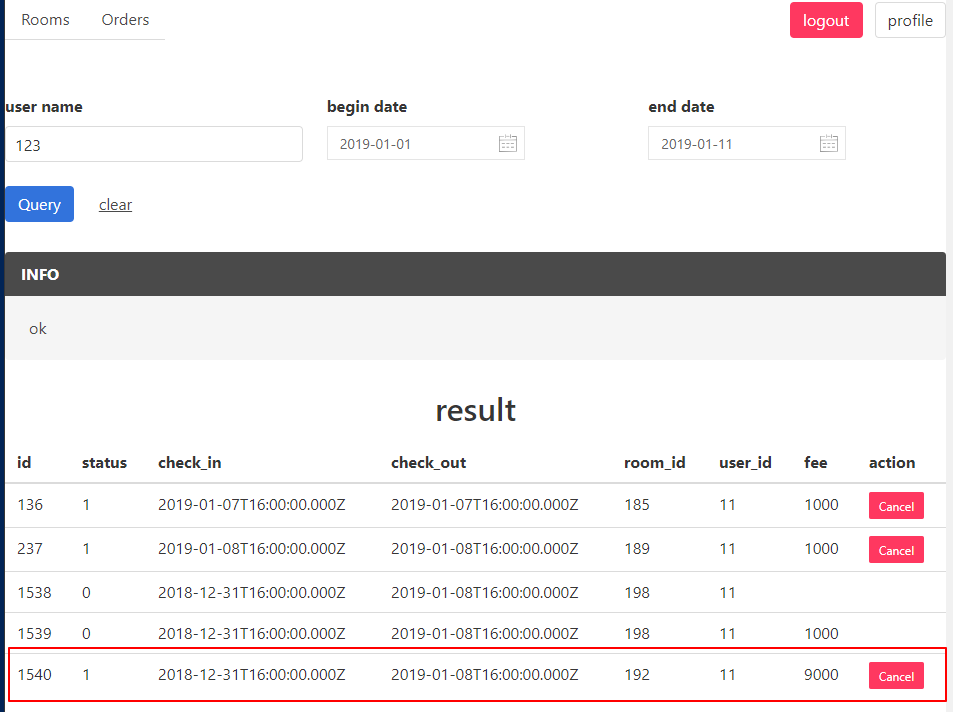
\includegraphics[width=15cm]{figure/2018-12-22-15-30-21.png}
    \caption{查看订单}
    \label{fig:order_room_2}
    %\end{adjustwidth}
\end{figure}

可以看到,由于定了9天,因此系统生成的订单里也的确生成了9*1000=9000元的订单,同时用户的余额少了9000,可见\autoref{fig:order_room_3}。

%\usepackage{changepage}
%\usepackage{rotating}
%\usepackage{float}
%\usepackage[section]{placeins}
%\begin{sidewaystable}[!Htp]
\begin{figure}[htp]
    %\begin{adjustwidth}{-1.5cm}{-1cm}
    \centering
    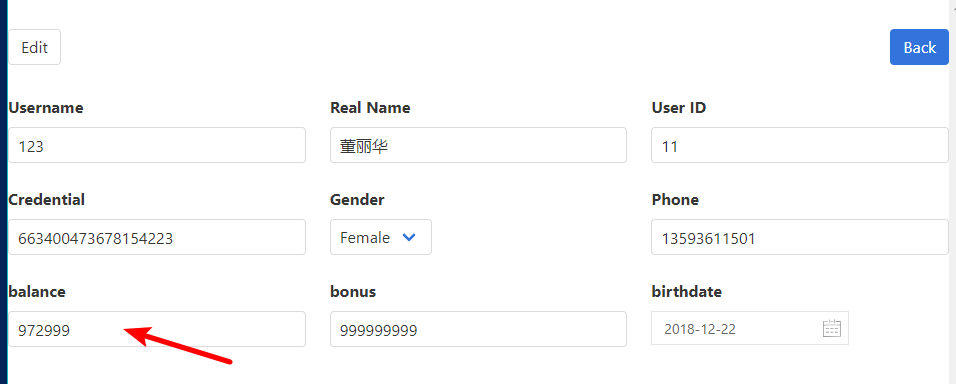
\includegraphics[width=10cm]{figure/2018-12-22-15-31-59.png}
    \caption{用户个人信息}
    \label{fig:order_room_3}
    %\end{adjustwidth}
\end{figure}



\chapter{开发所遇到的问题与解决方案}

% 这里描述一些我们在开发过程中遇到的问题
% TODO: 这个也许大家都来补充一下会好一些

在开发本数据库系统的过程中,我们遇到了很多问题,例如对可能改变数据库数据的一致性的用户请求该如何处理?在数据库增加一项如何自动生成id等。对这些开发细节的说明与解决,我们在下面分成了几个小节分别说明。

\section{如何保证数据一致性?}

在一些操作中,对于用户可能仅仅是一个点击的操作,但是在系统后台执行该请求时,往往需要涉及到多个对数据库的写操作。就以用户请求预定房间为例,该操作要求更新用户余额,更新Order表和Operation表等操作。

为了保证数据的一致性,需要将这些操作以事务的方式进行操作。在我们的实现中,有两种方式来实现事务,一种是在后端的代码中,使用数据库连接器提供的事务接口实现事务,可见\autoref{fig:dev-transaction-1}。

在另一种实现中,我们还编写了多个存储过程,在存储过程中使用“start transaction”,与“commit”语句实现事务操作,可见\autoref{procedure}。


%\usepackage{changepage}
%\usepackage{rotating}
%\usepackage{float}
%\usepackage[section]{placeins}
%\begin{sidewaystable}[!Htp]
\begin{figure}[htp]
    %\begin{adjustwidth}{-1.5cm}{-1cm}
    \centering
    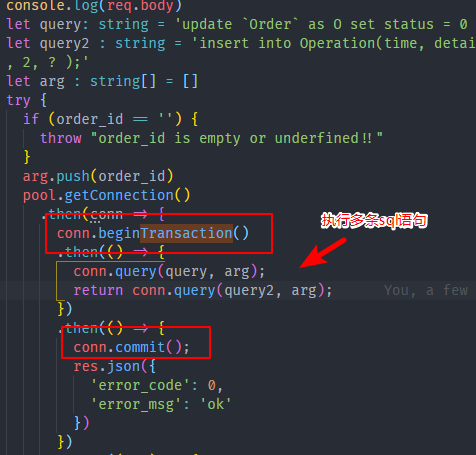
\includegraphics[width=7cm]{figure/2018-12-22-12-35-08.png}
    \caption{后端实现事务}
    \label{fig:dev-transaction-1}
    %\end{adjustwidth}
\end{figure}

\section{如何在查询订单时查询订单相关的操作明细?}

本次实验中网站后端使用的JavaScript语言采用了內建多个消息循环的执行模式向数据库发送一个查询
请求仅仅是将这一个查询请求“登记”到消息循环中,查询异步执行,程序将立即返回。因此,如果想在执行查询一个订单的查询语句中,直接嵌套另一个循环来查询操作明细是不可行的。解决方法有两种:

\begin{itemize}
    \item 使用事务机制,确保执行完所有语句后程序才返回
    \item 前端首先调用一次查询订单操作,再依据订单id查询操作明细
\end{itemize}

第一种方法更适合用来保证一致性。因此我们采用了第二种方法。


\section{用户权限的控制}

关于不同用户权限控制的实现,我们曾经有过争论,是在前后端层面处理用户的权限,还是使用数据库的用户权限机制来对不同用户的访问做限制呢?最终我们的方案采取了在前后端对用户的权限进行处理。在后端,我们使用了session中的信息进行了用户信息的检查,代码可见\autoref{fig:right-control},通过检查用户信息,能够做到本用户只能够查看本用户的信息,在其他接口中,也是用了类似的方法对权限进行了检查,以防止没有登录的人,或者权限较低的用户通过直接访问api的方式获取数据库的数据。

%\usepackage{changepage}
%\usepackage{rotating}
%\usepackage{float}
%\usepackage[section]{placeins}
%\begin{sidewaystable}[!Htp]
\begin{figure}[htp]
    %\begin{adjustwidth}{-1.5cm}{-1cm}
    \centering
    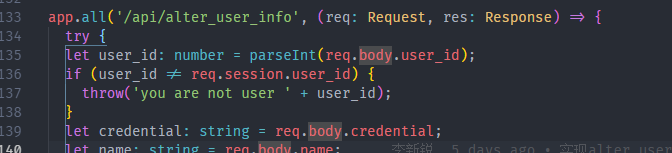
\includegraphics[width=10cm]{figure/2018-12-22-13-03-10.png}
    \caption{用户权限控制在后端的实现}
    \label{fig:right-control}
    %\end{adjustwidth}
\end{figure}

\section{存储过程的传参和返回值}
存储过程相当于是存储并编译在数据库中的一段子程序。它在传参和返回值上和一般的查询语句都有所不同:

在查询房间时,用户如果不对是否提供wifi、早餐做出要求,那么就应该既返回提供wifi的房间,又返回不提供wifi的房间。我们发现可以使用like谓词实现这个需求:\textit{where \space wifi \space like \space '\%'} 。但在把这条查询语句写入存储过程时发生了问题,实验发现:存储过程在传参过程中不允许参数发生隐式类型转换,如果把参数Arg\_wifi声明为bool,那么刚刚这条查询语句就会出错,因此必须将参数Arg\_wifi声明为char(1)。

此外存储过程的返回值在后端中是list of list,而一般的查询语句的返回值是list。这一点也要特殊处理。


\section{NULL与数字比较}
实验发现:如果一个属性num的值为\textit{null},那么它或它的与其他数字运算的结果出现在if语句中和其他数字比较,if语句均会返回false。因此在判断用户余额是否足够订房时最好要检查余额是否为\textit{null},避免由于数据库数据上的失误出现部分用户可以无限订房的情况。

% TODO: 补充一些问题?? 有一些开发细节可能会好一些

%%%%%%%%%%%%%%%%%%%%%%%%%%%%%%%%%%%%%%%%%%%%%%%%%%%%%%%%%%%%%%%%%%%%%%%%%%%%
% 参考文献
%%%%%%%%%%%%%%%%%%%%%%%%%%%%%%%%%%%%%%%%%%%%%%%%%%%%%%%%%%%%%%%%%%%%%%%%%%%%
% \cleardoublepage\phantomsection
% \addcontentsline{toc}{chapter}{参考文献}

% \bibliography{opsystem}
% \bibliographystyle{unsrt}

% \begin{thebibliography}{00}
%   \bibitem{r1} 作者. 文章题目 [J].  期刊名, 出版年份,卷号(期数): 起止页码.
%   \bibitem{r2} 作者. 书名 [M]. 版次. 出版地:出版单位,出版年份:起止页码.
%   \bibitem{r3} 邓建松等, 《\LaTeXe~科技排版指南》, 科学出版社.
%   \bibitem{r4} 吴凌云, 《CTeX~FAQ (常见问题集)》, \textit{Version~0.4}, June 21, 2004.
%   \bibitem{r5} Herbert Vo\ss, Mathmode, \url{http://www.tex.ac.uk/ctan/info/math/voss/mathmode/Mathmode.pdf}.
% \end{thebibliography}
%%%%%%%%%%%%%%%%%%%%%%%%%%%%%%%%%%%%%%%%%%%%%%%%%%%%%%%%%%%%%%%%%%%%%%%%%%%%
% 附录
%%%%%%%%%%%%%%%%%%%%%%%%%%%%%%%%%%%%%%%%%%%%%%%%%%%%%%%%%%%%%%%%%%%%%%%%%%%%
\appendix


\cleardoublepage
\end{document}
